
	\subsection{2.10. Неприводимые представления и характер представления. Формула приведения.} 
	
	\par\bigskip
	
	Матрицы, соответствующие операциям в точечных группах в
	базисе орбиталей обычно получаются большой размерности,
	оперировать ими неудобно. С помощью подходящего
	преобразования подобия можно превратить обычную матрицу в
	блочно-диагональную. В такой матрице ненулевые элементы
	сгруппированы только в квадратных блоках, расположенных вдоль
	главной диагонали. Достоинства таких матриц лучшего всего
	проявляются при их умножении. В общем виде, если две матрицы
	А и Б с помощью преобразования подобия могут быть приведены к
	блочно-диагональным матрицам, имеющим одинаковую форму, их
	произведение В имеет аналогичный вид:
	
		\begin{figure}[H]
		\centering
		{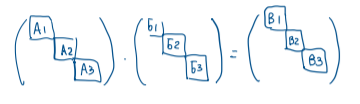
\includegraphics[scale=1.5]{35.png}}
	\end{figure}
	
	
	Операция умножения справедлива и для индивидиуальных блоков:
	
		\begin{figure}[H]
		\centering
		{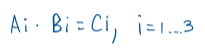
\includegraphics[scale=1.5]{36.png}}
	\end{figure}
	
	
	
	Получается, что представлением некоторой операции симметрии
	будет являться не только полная матрица В, но и малые В1, В2, В3.
	
		\par\smallskip
	
	
	Если предположить, что матрицы А, Б и В (и единичная матрица)
	образуют представление для некоторой точечной группы
	симметрии, то это называется приводимым представлением
	группы, поскольку для приведения матриц существует
	преобразование подобия. Затем каждый из индивидуальных блоков
	упрощают преобразованием подобия до тех пор, пока вдоль
	диагонали каждой из больших матриц не появятся простейшие
	блоки. Это состояние будет соответствовать неприводимым
	представлениям. В таком случае каждый набор малых матриц,
	сгруппированных вдоль диагоналей больших матриц ({Ai, Bi, Ci})
	будет неприводимым представлением данной точечной группы.
	Таким образом, в данном примере приводимое представление
	распалось на три неприводимых.
	
		\par\smallskip
	
	
	Вместо работы с неприводимыми представлениями можно
	использовать их характеры. Характер матрицы - это сумма ее
	диагональных элементов. Для любого представления характер
	представления является совокупностью характеров всех матриц в
	данной точечной группе. Таким образом, характер некоторого
	представления будет просто являться совокупностью чисел. Однако
	может быть неясно, приводимо или неприводимо такое
	представление. Для этого надо знать характеры неприводимых
	представлений данной точечной группы. Характеры неприводимых
	представлений сведены в специальные таблицы характеров. Если
	какое-либо представление в данной точечной группе там не
	имеется, то оно приводимое и может быть сведено к линейной
	комбинации неприводимых представлений. Иногда это легко
	увидеть и так, но для больших таблиц выгоднее использовать
	формулу приведения.
	
	
		\par\smallskip
	
	
	Разложение любого приводимого представления может быть
	осуществлено единственным способом. К конечным точечным
	группам (не к ) можно применять формулу
	приведения. Она позволяет понять, как некоторое приводимое
	представление раскладывается на неприводимые. 
	
		\begin{figure}[H]
		\centering
		{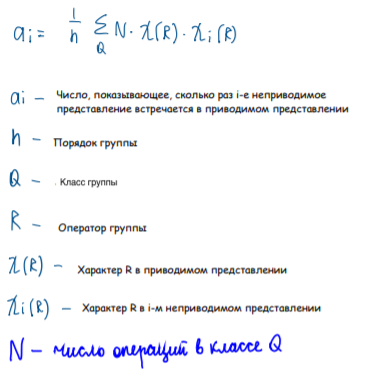
\includegraphics[scale=1.5]{37.png}}
	\end{figure}
	
	\par\bigskip
	\par\bigskip
	